
\begin{figure}
    \centering
\begin{subfigure}[b]{0.33\textwidth} 
  \centering 
  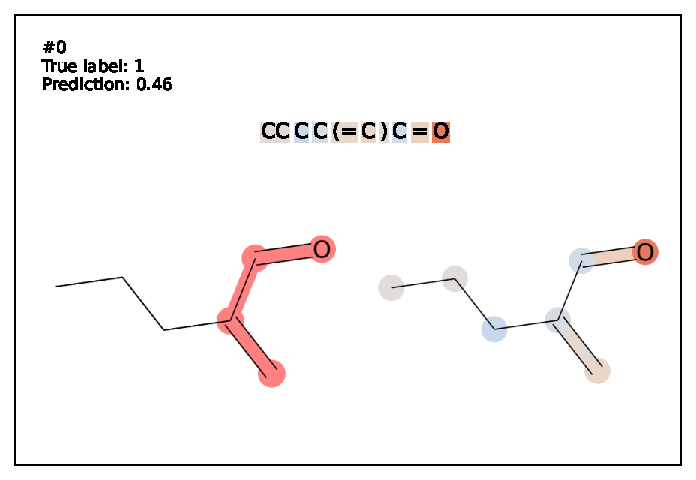
\includegraphics[width=\textwidth]{figures/ames/ames0.pdf} 
\end{subfigure}\begin{subfigure}[b]{0.33\textwidth} 
  \centering 
  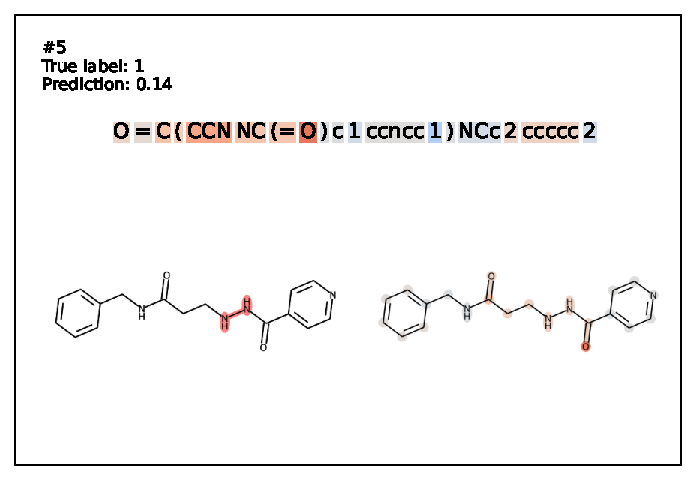
\includegraphics[width=\textwidth]{figures/ames/ames5.pdf} 
\end{subfigure}\begin{subfigure}[b]{0.33\textwidth} 
  \centering 
  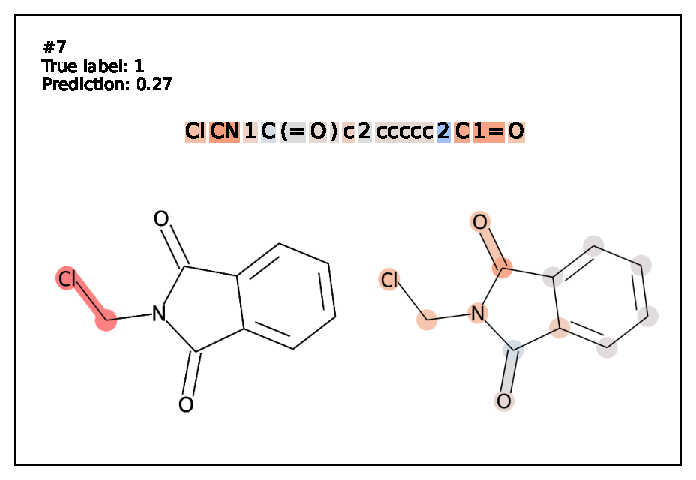
\includegraphics[width=\textwidth]{figures/ames/ames7.pdf} 
\end{subfigure} 
\begin{subfigure}[b]{0.33\textwidth} 
  \centering 
  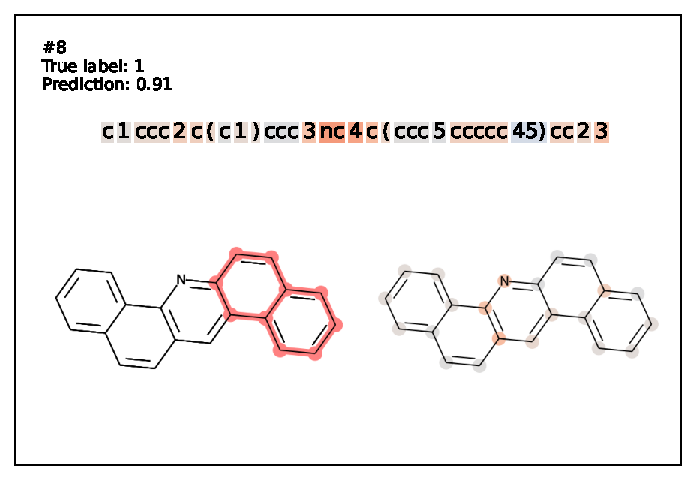
\includegraphics[width=\textwidth]{figures/ames/ames8.pdf} 
\end{subfigure}\begin{subfigure}[b]{0.33\textwidth} 
  \centering 
  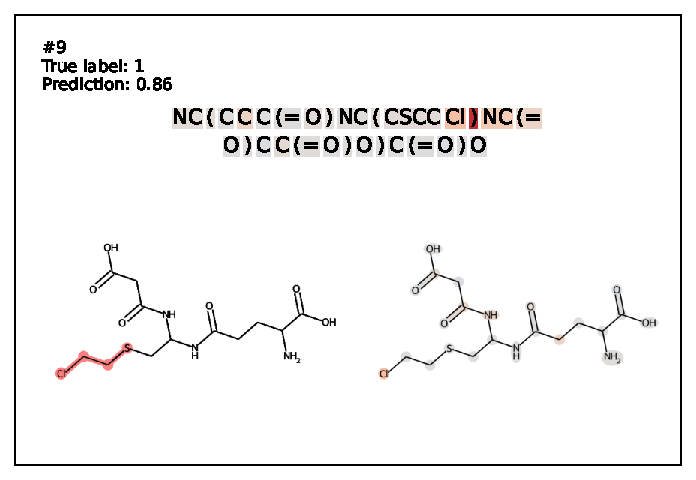
\includegraphics[width=\textwidth]{figures/ames/ames9.pdf} 
\end{subfigure}\begin{subfigure}[b]{0.33\textwidth} 
  \centering 
  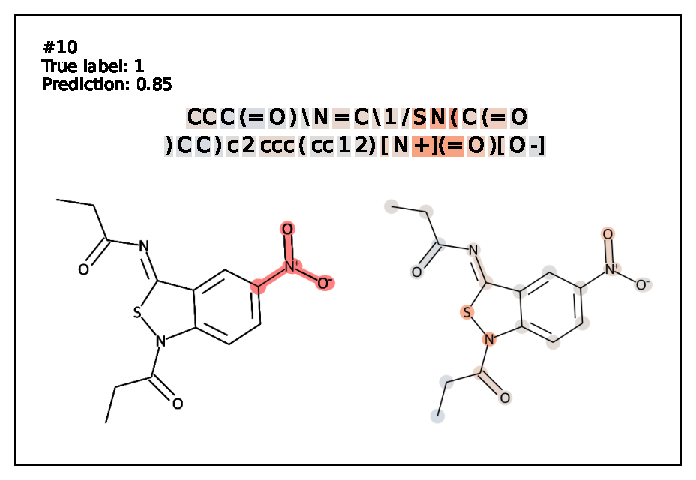
\includegraphics[width=\textwidth]{figures/ames/ames10.pdf} 
\end{subfigure} 
\begin{subfigure}[b]{0.33\textwidth} 
  \centering 
  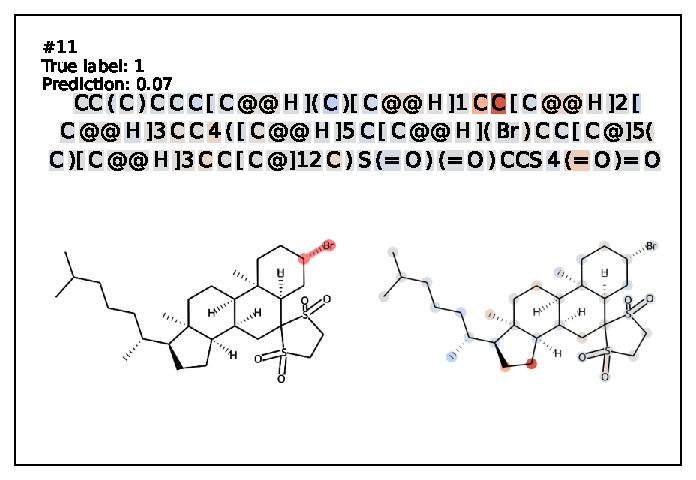
\includegraphics[width=\textwidth]{figures/ames/ames11.pdf} 
\end{subfigure}\begin{subfigure}[b]{0.33\textwidth} 
  \centering 
  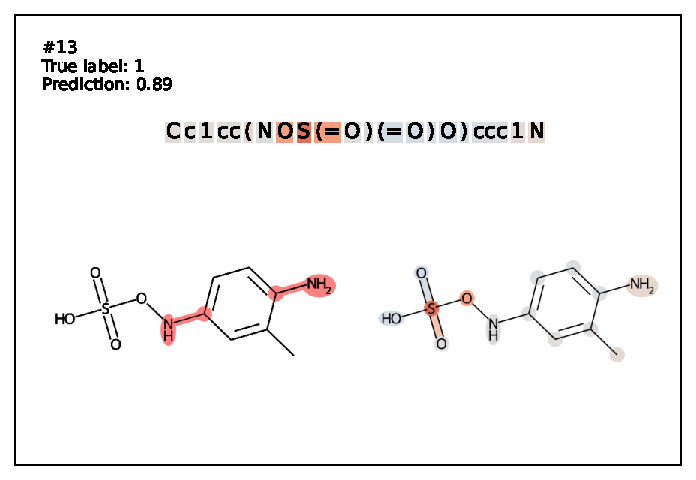
\includegraphics[width=\textwidth]{figures/ames/ames13.pdf} 
\end{subfigure}\begin{subfigure}[b]{0.33\textwidth} 
  \centering 
  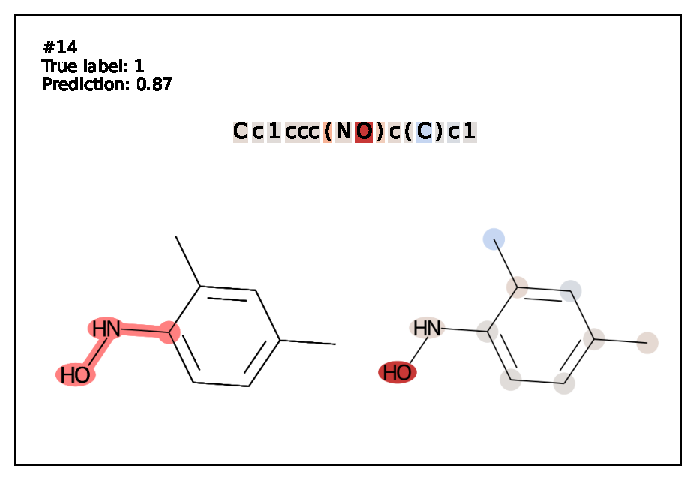
\includegraphics[width=\textwidth]{figures/ames/ames14.pdf} 
\end{subfigure} 
\begin{subfigure}[b]{0.33\textwidth} 
  \centering 
  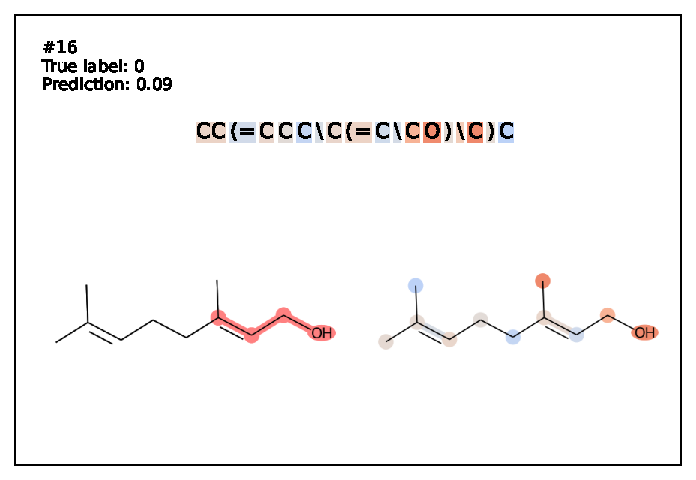
\includegraphics[width=\textwidth]{figures/ames/ames16.pdf} 
\end{subfigure}\begin{subfigure}[b]{0.33\textwidth} 
  \centering 
  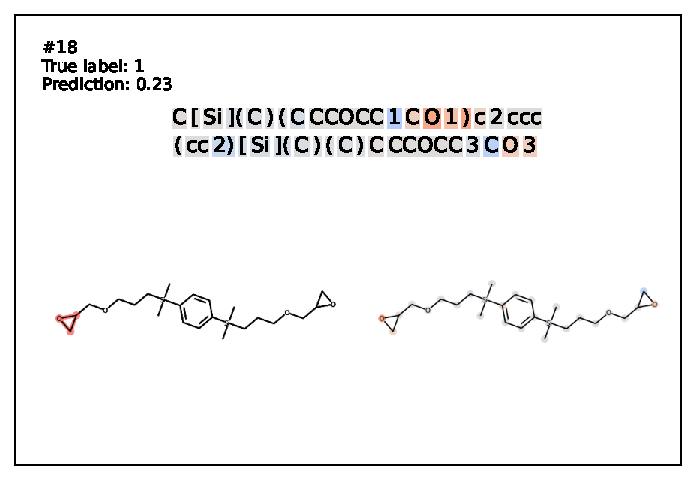
\includegraphics[width=\textwidth]{figures/ames/ames18.pdf} 
\end{subfigure}\begin{subfigure}[b]{0.33\textwidth} 
  \centering 
  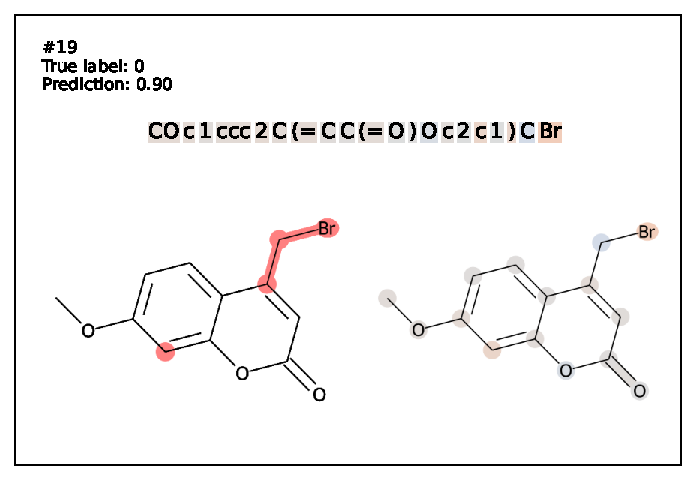
\includegraphics[width=\textwidth]{figures/ames/ames19.pdf} 
\end{subfigure} 
\begin{subfigure}[b]{0.33\textwidth} 
  \centering 
  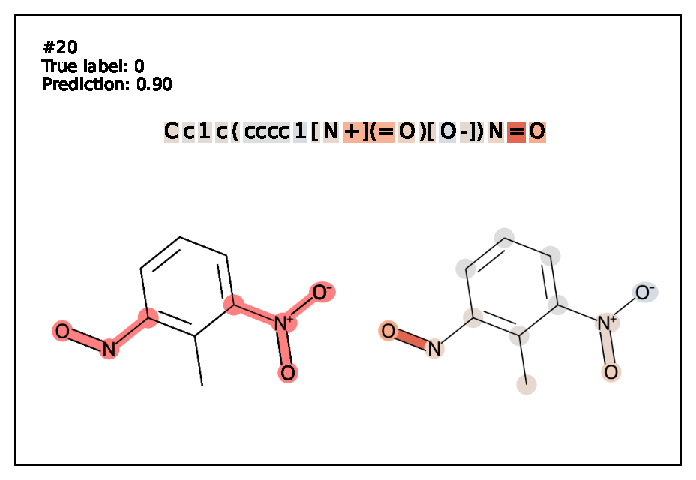
\includegraphics[width=\textwidth]{figures/ames/ames20.pdf} 
\end{subfigure}\begin{subfigure}[b]{0.33\textwidth} 
  \centering 
  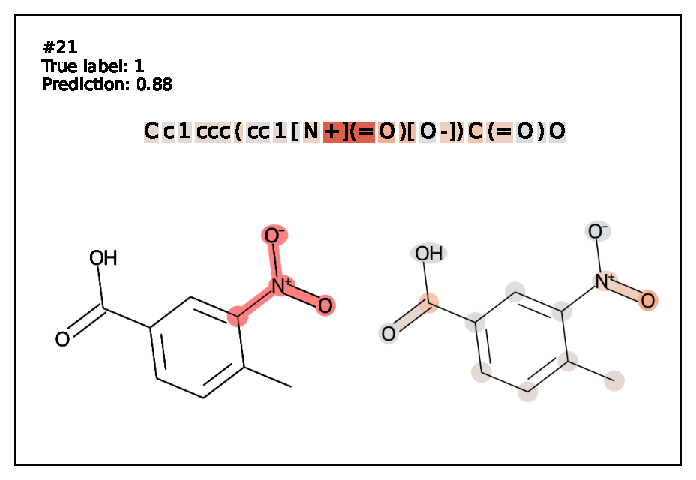
\includegraphics[width=\textwidth]{figures/ames/ames21.pdf} 
\end{subfigure}\begin{subfigure}[b]{0.33\textwidth} 
  \centering 
  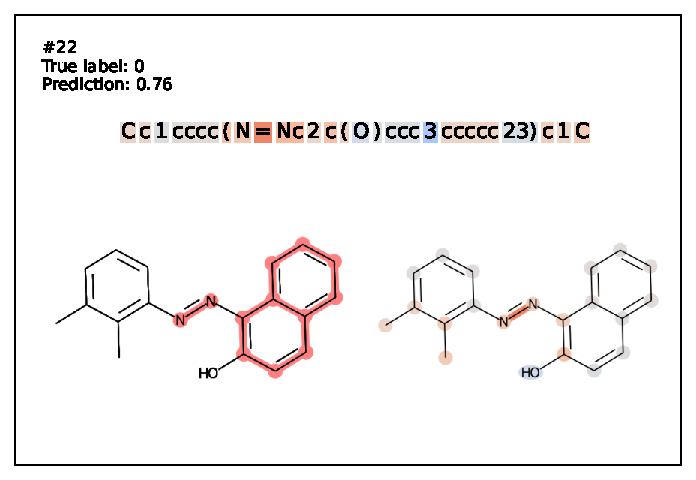
\includegraphics[width=\textwidth]{figures/ames/ames22.pdf} 
\end{subfigure} 
\begin{subfigure}[b]{0.33\textwidth} 
  \centering 
  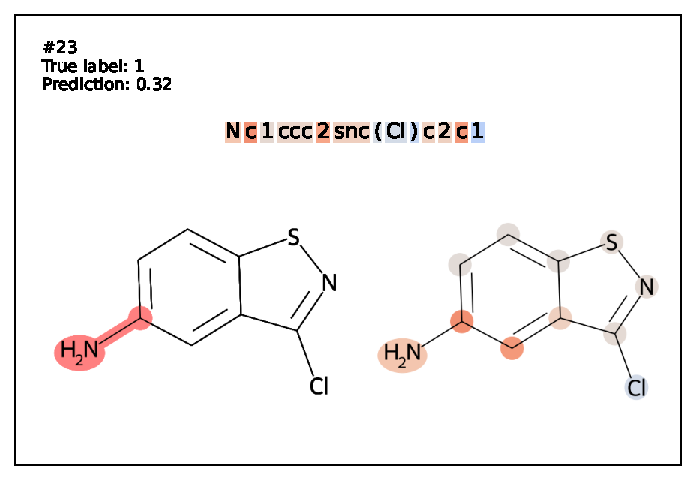
\includegraphics[width=\textwidth]{figures/ames/ames23.pdf} 
\end{subfigure}\begin{subfigure}[b]{0.33\textwidth} 
  \centering 
  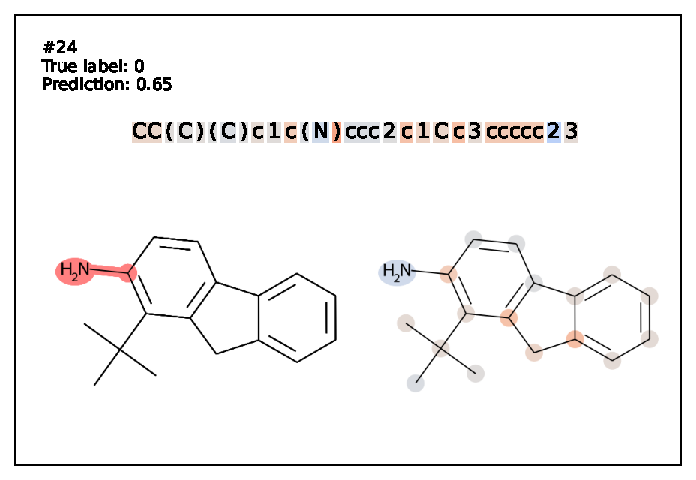
\includegraphics[width=\textwidth]{figures/ames/ames24.pdf} 
\end{subfigure}\begin{subfigure}[b]{0.33\textwidth} 
  \centering 
  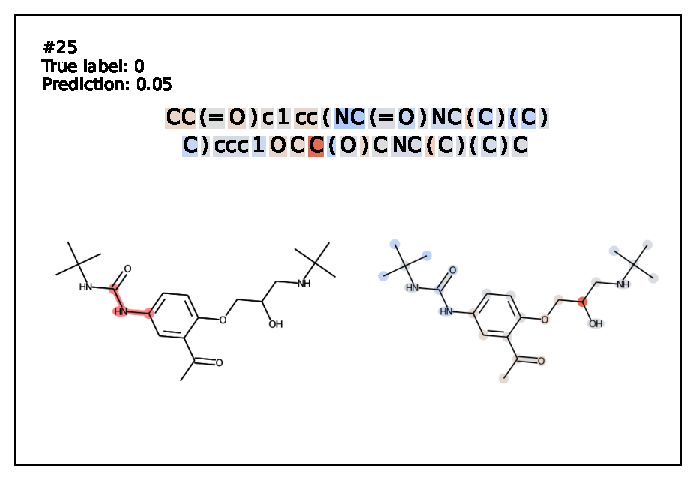
\includegraphics[width=\textwidth]{figures/ames/ames25.pdf} 
\end{subfigure} 
\begin{subfigure}[b]{0.33\textwidth} 
  \centering 
  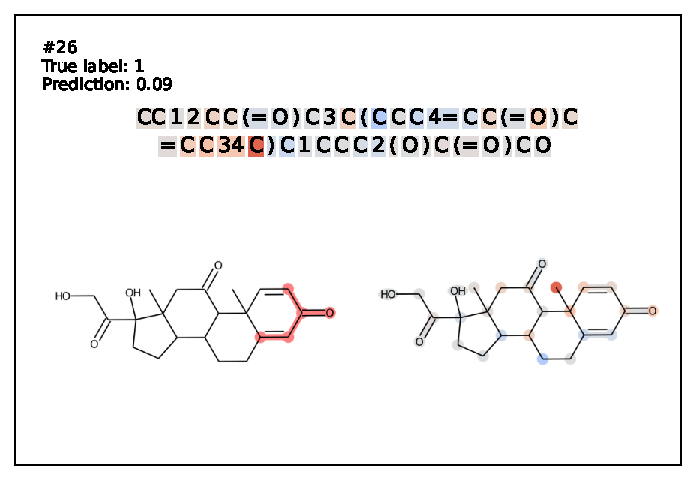
\includegraphics[width=\textwidth]{figures/ames/ames26.pdf} 
\end{subfigure}\begin{subfigure}[b]{0.33\textwidth} 
  \centering 
  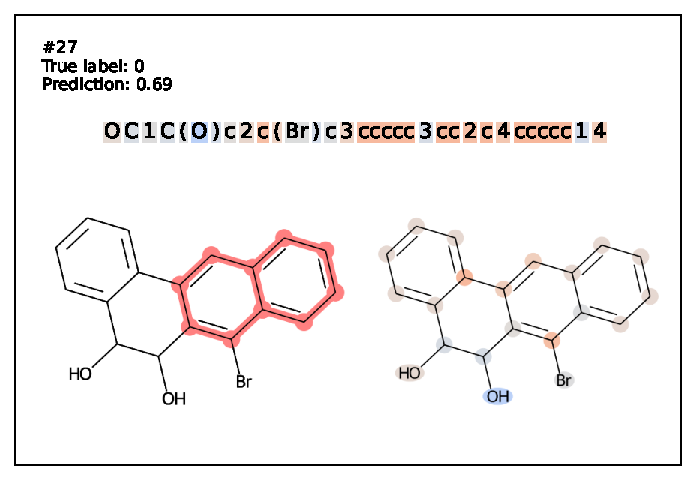
\includegraphics[width=\textwidth]{figures/ames/ames27.pdf} 
\end{subfigure}\begin{subfigure}[b]{0.33\textwidth} 
  \centering 
  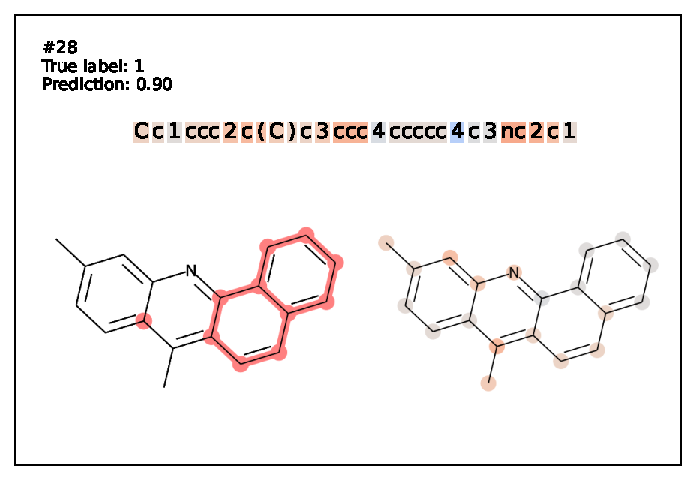
\includegraphics[width=\textwidth]{figures/ames/ames28.pdf} 
\end{subfigure} 
\caption{Explaining predictions of the fine-tuned model on Ames dataset. See Section \ref{sec:captum}. Part 1/5}
\label{fig:captum-ames-1}
\end{figure}

\begin{figure}
\centering
\begin{subfigure}[b]{0.33\textwidth} 
  \centering 
  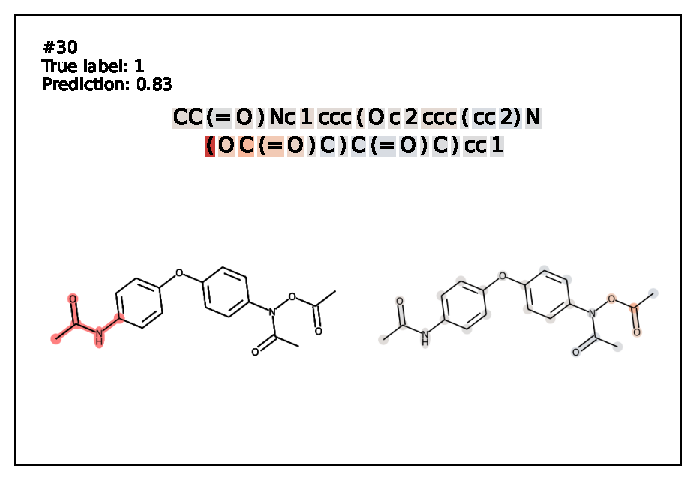
\includegraphics[width=\textwidth]{figures/ames/ames30.pdf} 
\end{subfigure}\begin{subfigure}[b]{0.33\textwidth} 
  \centering 
  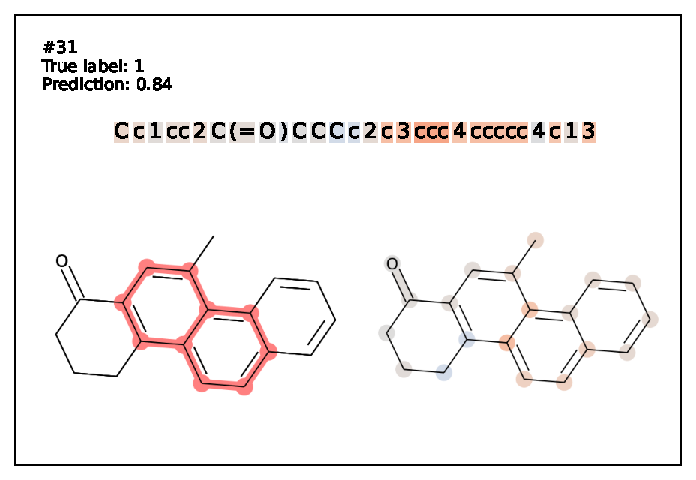
\includegraphics[width=\textwidth]{figures/ames/ames31.pdf} 
\end{subfigure}\begin{subfigure}[b]{0.33\textwidth} 
  \centering 
  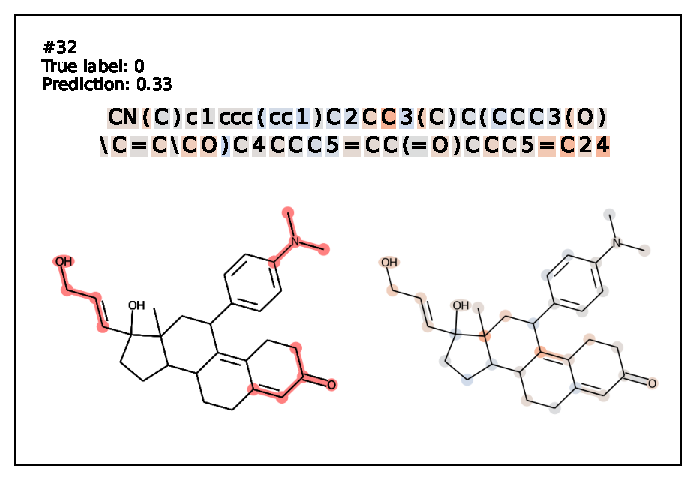
\includegraphics[width=\textwidth]{figures/ames/ames32.pdf} 
\end{subfigure} 
\begin{subfigure}[b]{0.33\textwidth} 
  \centering 
  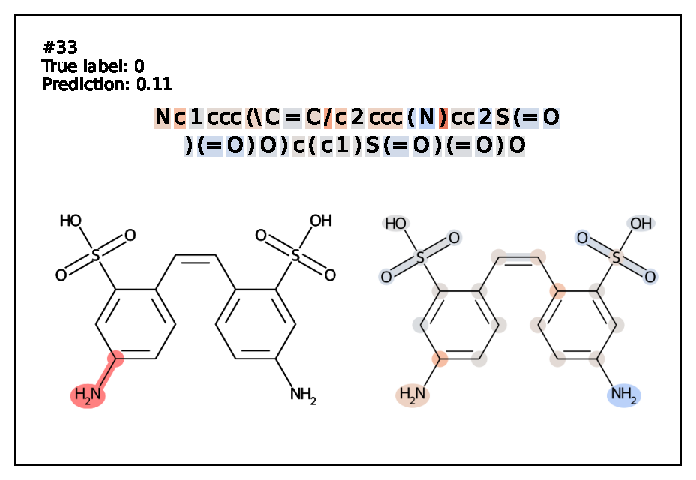
\includegraphics[width=\textwidth]{figures/ames/ames33.pdf} 
\end{subfigure}\begin{subfigure}[b]{0.33\textwidth} 
  \centering 
  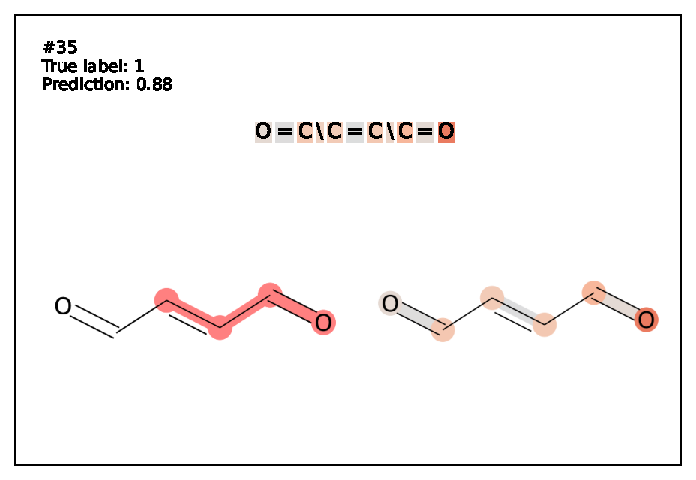
\includegraphics[width=\textwidth]{figures/ames/ames35.pdf} 
\end{subfigure}\begin{subfigure}[b]{0.33\textwidth} 
  \centering 
  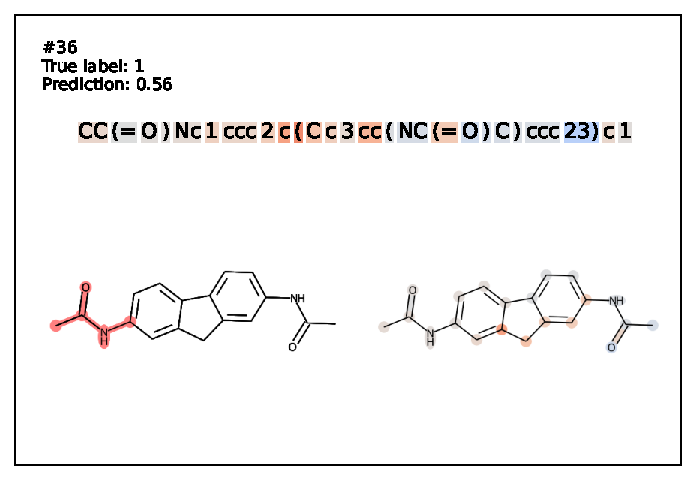
\includegraphics[width=\textwidth]{figures/ames/ames36.pdf} 
\end{subfigure} 
\begin{subfigure}[b]{0.33\textwidth} 
  \centering 
  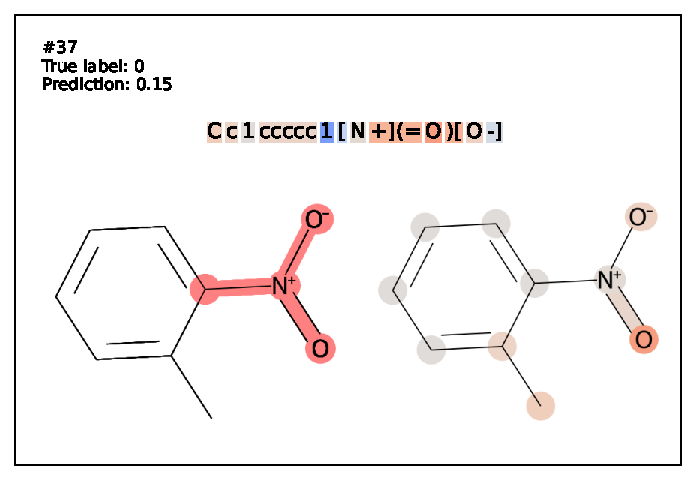
\includegraphics[width=\textwidth]{figures/ames/ames37.pdf} 
\end{subfigure}\begin{subfigure}[b]{0.33\textwidth} 
  \centering 
  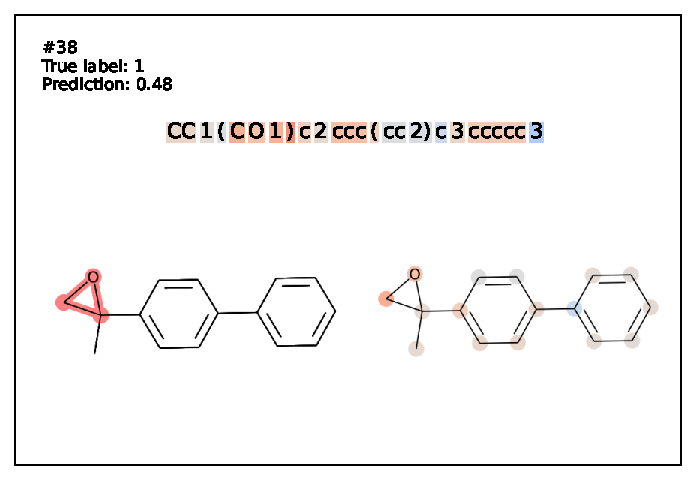
\includegraphics[width=\textwidth]{figures/ames/ames38.pdf} 
\end{subfigure}\begin{subfigure}[b]{0.33\textwidth} 
  \centering 
  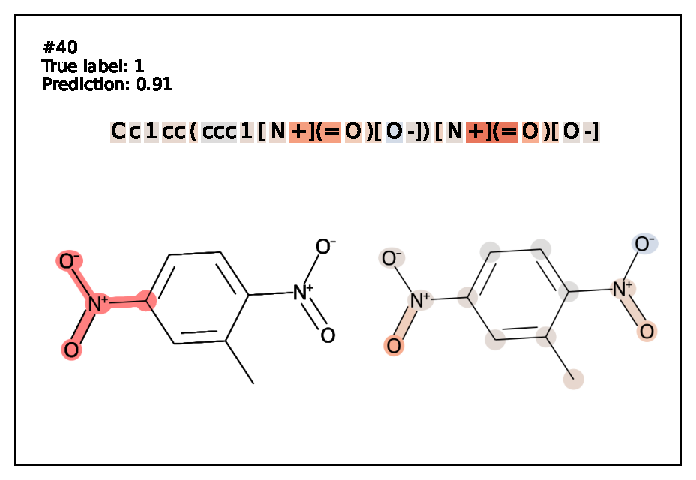
\includegraphics[width=\textwidth]{figures/ames/ames40.pdf} 
\end{subfigure} 
\begin{subfigure}[b]{0.33\textwidth} 
  \centering 
  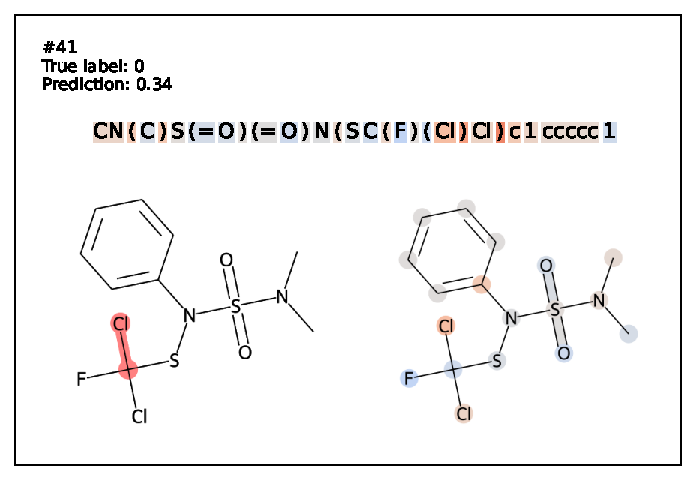
\includegraphics[width=\textwidth]{figures/ames/ames41.pdf} 
\end{subfigure}\begin{subfigure}[b]{0.33\textwidth} 
  \centering 
  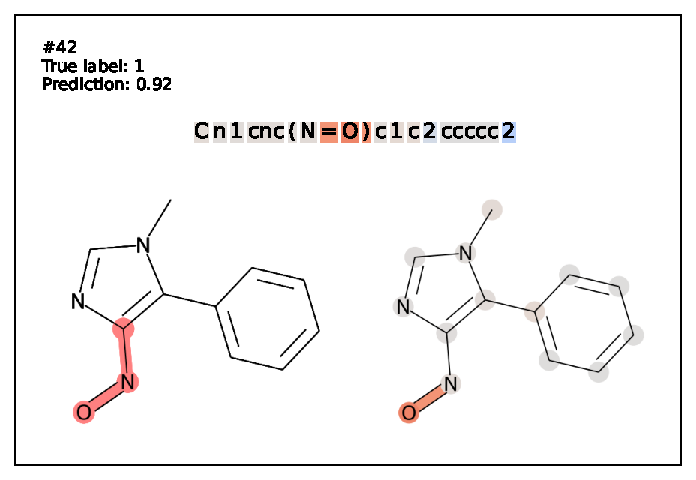
\includegraphics[width=\textwidth]{figures/ames/ames42.pdf} 
\end{subfigure}\begin{subfigure}[b]{0.33\textwidth} 
  \centering 
  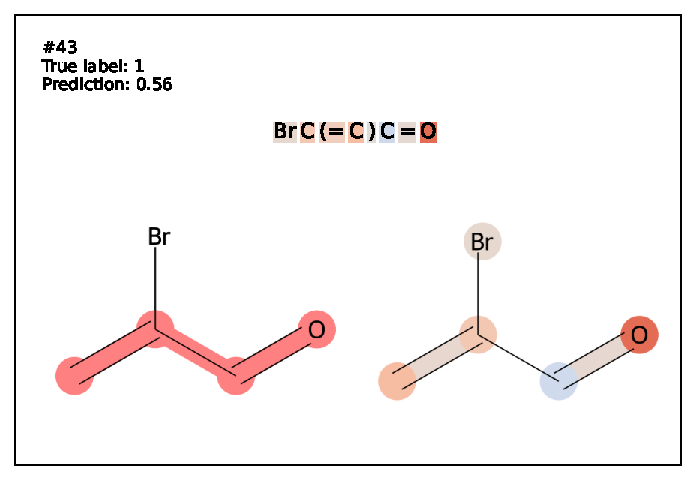
\includegraphics[width=\textwidth]{figures/ames/ames43.pdf} 
\end{subfigure} 
\begin{subfigure}[b]{0.33\textwidth} 
  \centering 
  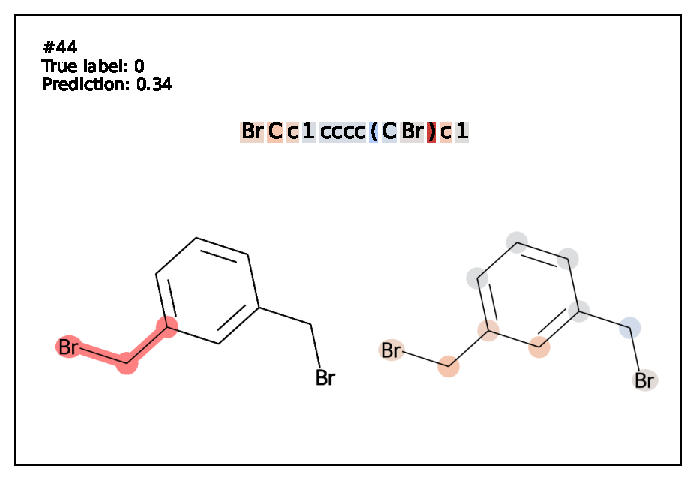
\includegraphics[width=\textwidth]{figures/ames/ames44.pdf} 
\end{subfigure}\begin{subfigure}[b]{0.33\textwidth} 
  \centering 
  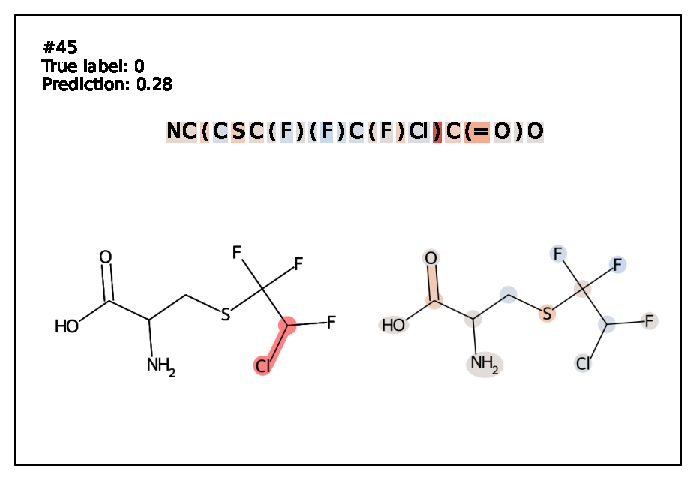
\includegraphics[width=\textwidth]{figures/ames/ames45.pdf} 
\end{subfigure}\begin{subfigure}[b]{0.33\textwidth} 
  \centering 
  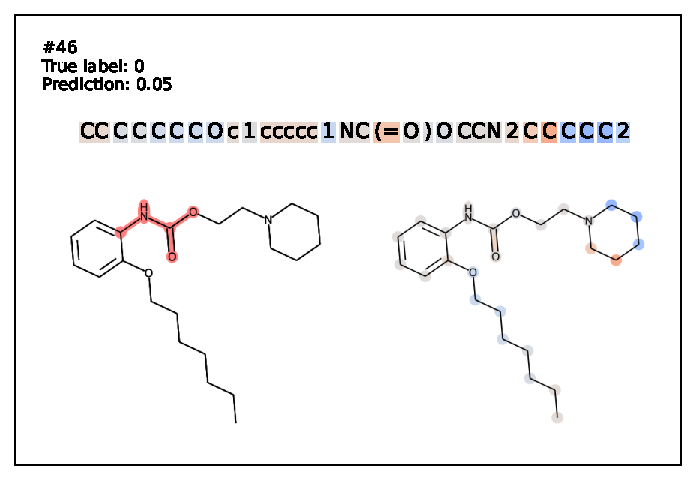
\includegraphics[width=\textwidth]{figures/ames/ames46.pdf} 
\end{subfigure} 
\begin{subfigure}[b]{0.33\textwidth} 
  \centering 
  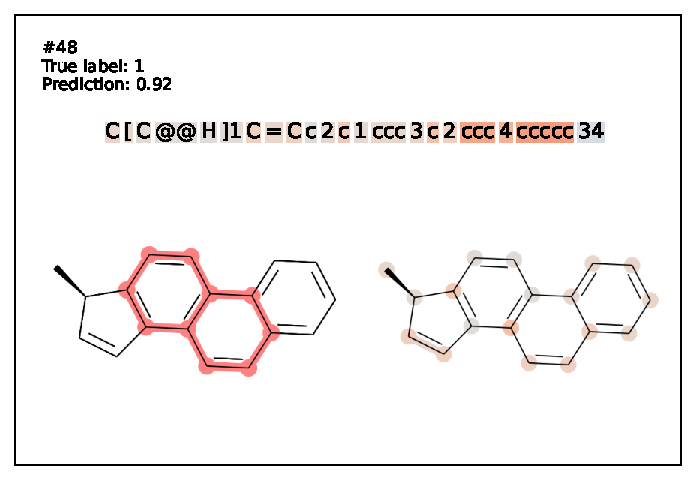
\includegraphics[width=\textwidth]{figures/ames/ames48.pdf} 
\end{subfigure}\begin{subfigure}[b]{0.33\textwidth} 
  \centering 
  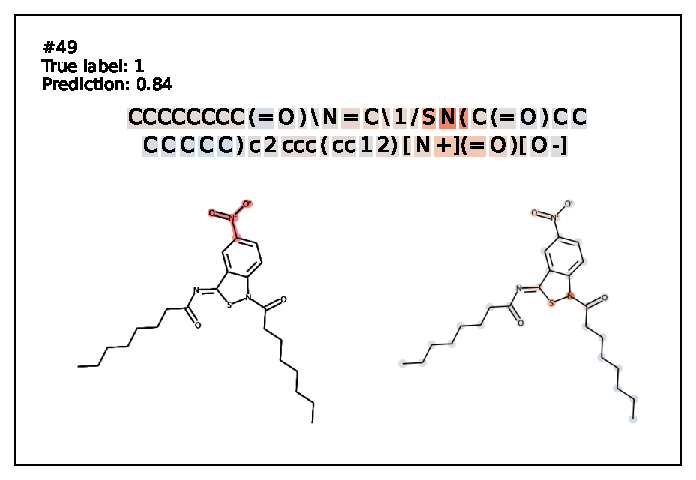
\includegraphics[width=\textwidth]{figures/ames/ames49.pdf} 
\end{subfigure}\begin{subfigure}[b]{0.33\textwidth} 
  \centering 
  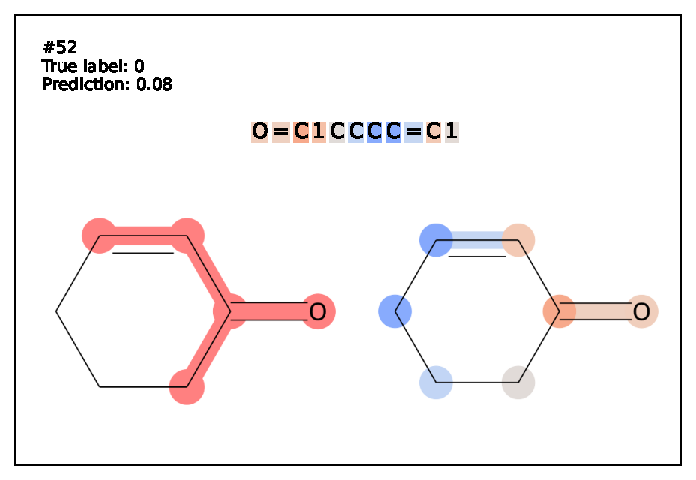
\includegraphics[width=\textwidth]{figures/ames/ames52.pdf} 
\end{subfigure} 
\begin{subfigure}[b]{0.33\textwidth} 
  \centering 
  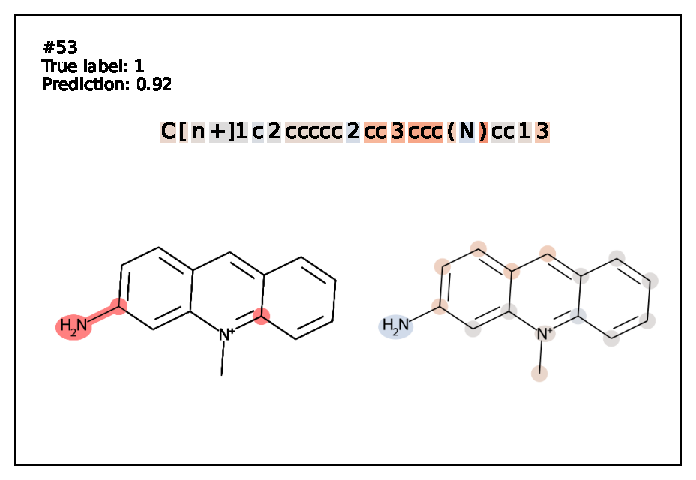
\includegraphics[width=\textwidth]{figures/ames/ames53.pdf} 
\end{subfigure}\begin{subfigure}[b]{0.33\textwidth} 
  \centering 
  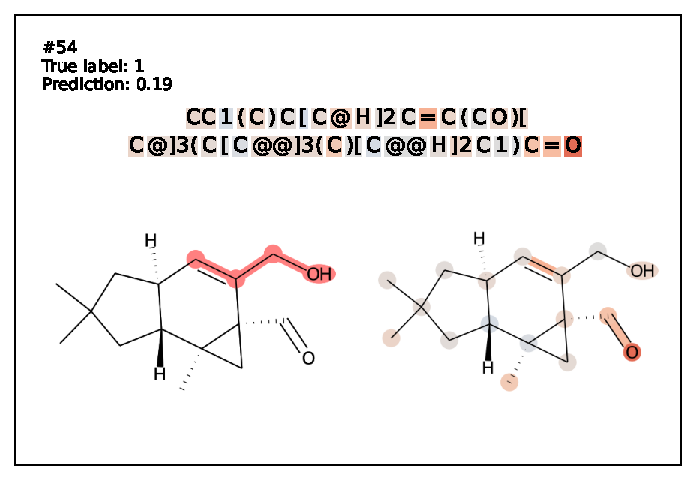
\includegraphics[width=\textwidth]{figures/ames/ames54.pdf} 
\end{subfigure}\begin{subfigure}[b]{0.33\textwidth} 
  \centering 
  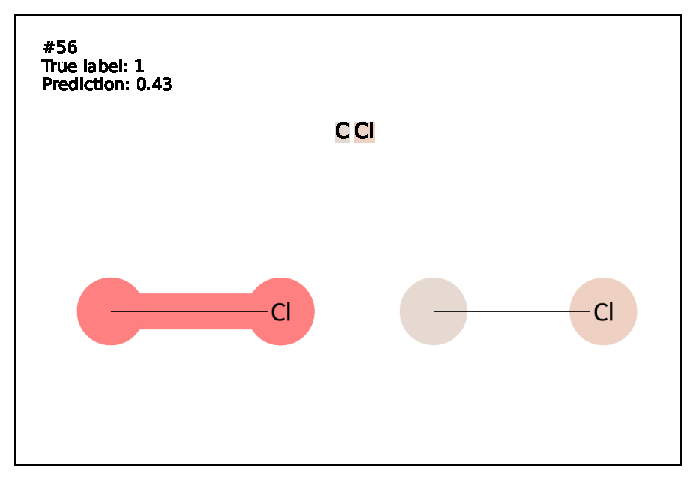
\includegraphics[width=\textwidth]{figures/ames/ames56.pdf} 
\end{subfigure} 
\caption{Explaining predictions of the fine-tuned model on Ames dataset. See Section \ref{sec:captum}. Part 2/5}
\label{fig:captum-ames-2}
\end{figure}

\begin{figure}
\centering
\begin{subfigure}[b]{0.33\textwidth} 
  \centering 
  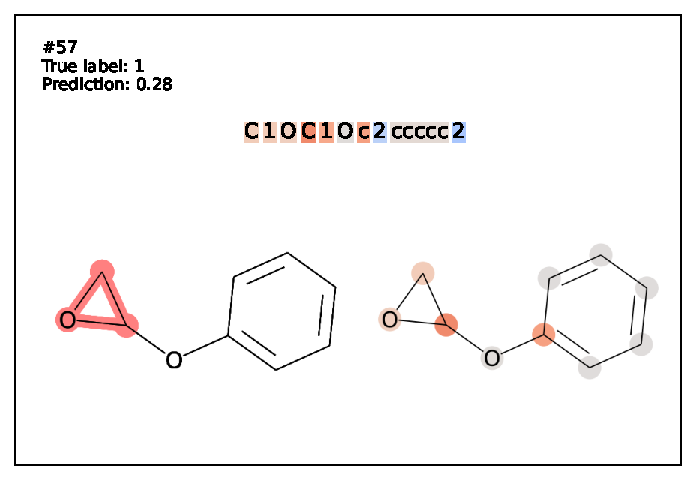
\includegraphics[width=\textwidth]{figures/ames/ames57.pdf} 
\end{subfigure}\begin{subfigure}[b]{0.33\textwidth} 
  \centering 
  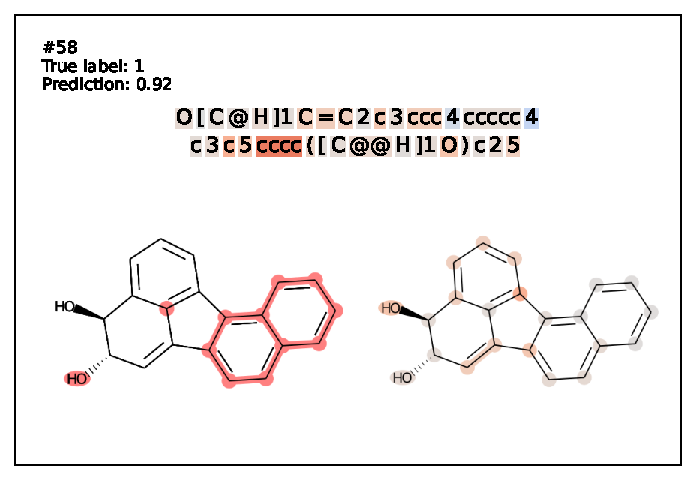
\includegraphics[width=\textwidth]{figures/ames/ames58.pdf} 
\end{subfigure}\begin{subfigure}[b]{0.33\textwidth} 
  \centering 
  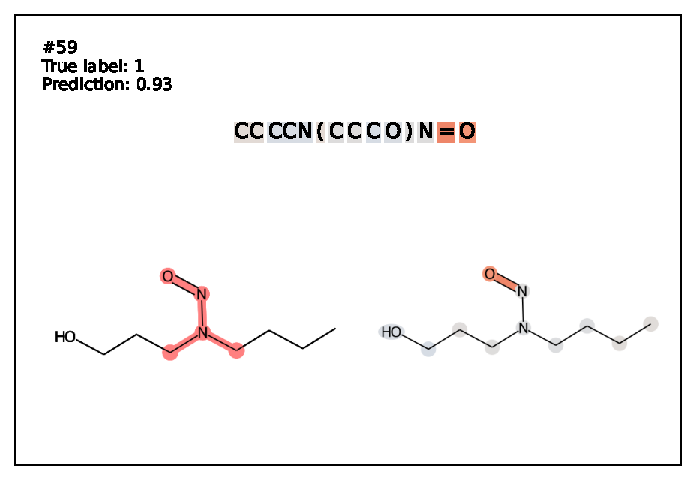
\includegraphics[width=\textwidth]{figures/ames/ames59.pdf} 
\end{subfigure} 
\begin{subfigure}[b]{0.33\textwidth} 
  \centering 
  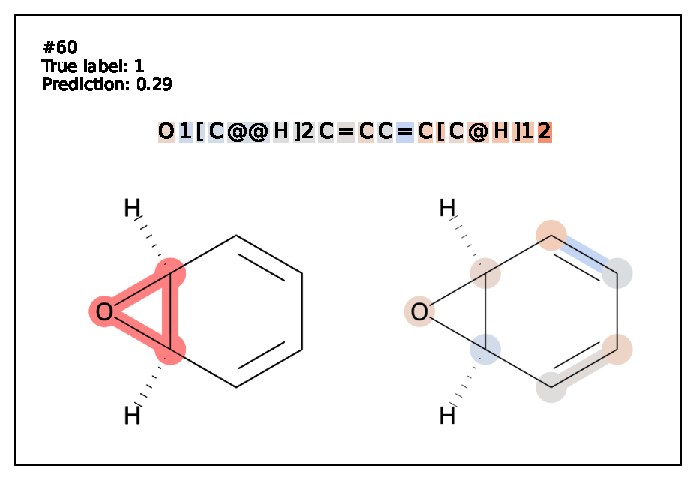
\includegraphics[width=\textwidth]{figures/ames/ames60.pdf} 
\end{subfigure}\begin{subfigure}[b]{0.33\textwidth} 
  \centering 
  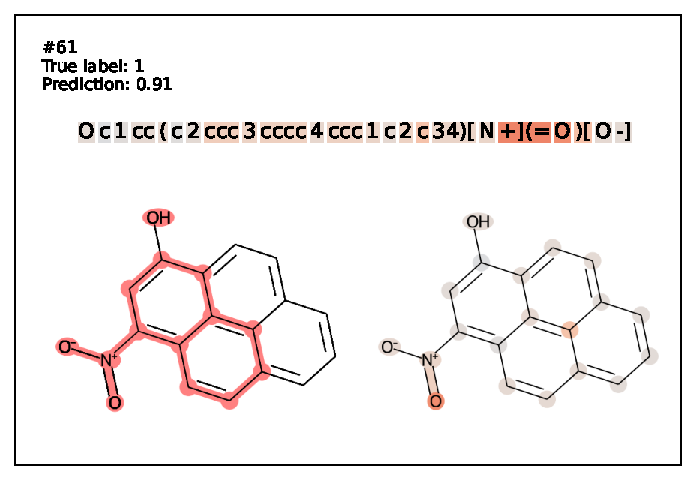
\includegraphics[width=\textwidth]{figures/ames/ames61.pdf} 
\end{subfigure}\begin{subfigure}[b]{0.33\textwidth} 
  \centering 
  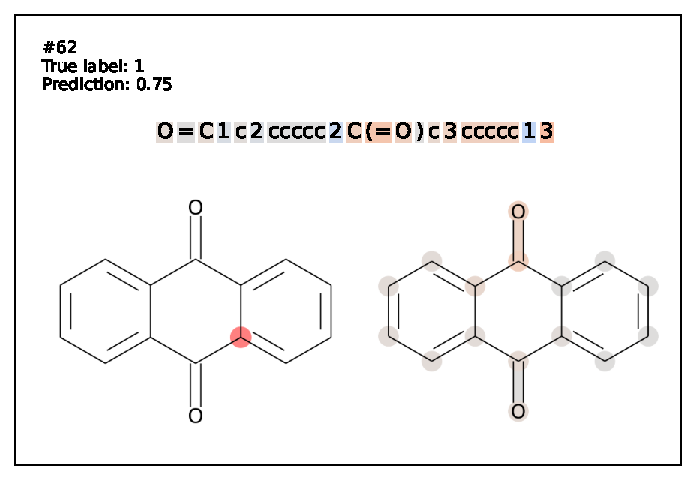
\includegraphics[width=\textwidth]{figures/ames/ames62.pdf} 
\end{subfigure} 
\begin{subfigure}[b]{0.33\textwidth} 
  \centering 
  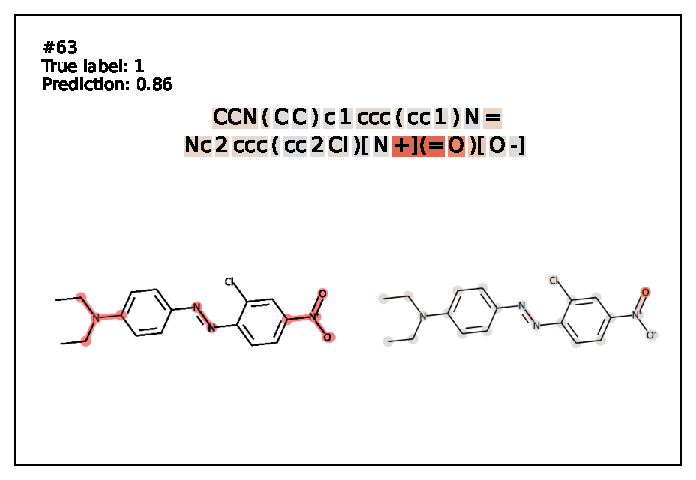
\includegraphics[width=\textwidth]{figures/ames/ames63.pdf} 
\end{subfigure}\begin{subfigure}[b]{0.33\textwidth} 
  \centering 
  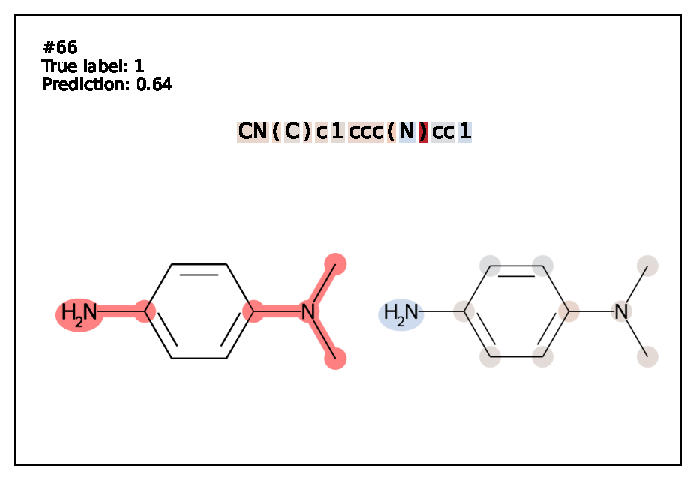
\includegraphics[width=\textwidth]{figures/ames/ames66.pdf} 
\end{subfigure}\begin{subfigure}[b]{0.33\textwidth} 
  \centering 
  \includegraphics[width=\textwidth]{figures/ames/ames69.pdf} 
\end{subfigure} 
\begin{subfigure}[b]{0.33\textwidth} 
  \centering 
  \includegraphics[width=\textwidth]{figures/ames/ames71.pdf} 
\end{subfigure}\begin{subfigure}[b]{0.33\textwidth} 
  \centering 
  \includegraphics[width=\textwidth]{figures/ames/ames73.pdf} 
\end{subfigure}\begin{subfigure}[b]{0.33\textwidth} 
  \centering 
  \includegraphics[width=\textwidth]{figures/ames/ames75.pdf} 
\end{subfigure} 
\begin{subfigure}[b]{0.33\textwidth} 
  \centering 
  \includegraphics[width=\textwidth]{figures/ames/ames76.pdf} 
\end{subfigure}\begin{subfigure}[b]{0.33\textwidth} 
  \centering 
  \includegraphics[width=\textwidth]{figures/ames/ames77.pdf} 
\end{subfigure}\begin{subfigure}[b]{0.33\textwidth} 
  \centering 
  \includegraphics[width=\textwidth]{figures/ames/ames78.pdf} 
\end{subfigure} 
\begin{subfigure}[b]{0.33\textwidth} 
  \centering 
  \includegraphics[width=\textwidth]{figures/ames/ames82.pdf} 
\end{subfigure}\begin{subfigure}[b]{0.33\textwidth} 
  \centering 
  \includegraphics[width=\textwidth]{figures/ames/ames83.pdf} 
\end{subfigure}\begin{subfigure}[b]{0.33\textwidth} 
  \centering 
  \includegraphics[width=\textwidth]{figures/ames/ames84.pdf} 
\end{subfigure} 
\begin{subfigure}[b]{0.33\textwidth} 
  \centering 
  \includegraphics[width=\textwidth]{figures/ames/ames86.pdf} 
\end{subfigure}\begin{subfigure}[b]{0.33\textwidth} 
  \centering 
  \includegraphics[width=\textwidth]{figures/ames/ames88.pdf} 
\end{subfigure}\begin{subfigure}[b]{0.33\textwidth} 
  \centering 
  \includegraphics[width=\textwidth]{figures/ames/ames89.pdf} 
\end{subfigure} 
\caption{Explaining predictions of the fine-tuned model on Ames dataset. See Section \ref{sec:captum}. Part 3/5}
\label{fig:captum-ames-3}
\end{figure}

\begin{figure}
\centering
\begin{subfigure}[b]{0.33\textwidth} 
  \centering 
  \includegraphics[width=\textwidth]{figures/ames/ames90.pdf} 
\end{subfigure}\begin{subfigure}[b]{0.33\textwidth} 
  \centering 
  \includegraphics[width=\textwidth]{figures/ames/ames91.pdf} 
\end{subfigure}\begin{subfigure}[b]{0.33\textwidth} 
  \centering 
  \includegraphics[width=\textwidth]{figures/ames/ames92.pdf} 
\end{subfigure} 
\begin{subfigure}[b]{0.33\textwidth} 
  \centering 
  \includegraphics[width=\textwidth]{figures/ames/ames93.pdf} 
\end{subfigure}\begin{subfigure}[b]{0.33\textwidth} 
  \centering 
  \includegraphics[width=\textwidth]{figures/ames/ames94.pdf} 
\end{subfigure}\begin{subfigure}[b]{0.33\textwidth} 
  \centering 
  \includegraphics[width=\textwidth]{figures/ames/ames95.pdf} 
\end{subfigure} 
\begin{subfigure}[b]{0.33\textwidth} 
  \centering 
  \includegraphics[width=\textwidth]{figures/ames/ames96.pdf} 
\end{subfigure}\begin{subfigure}[b]{0.33\textwidth} 
  \centering 
  \includegraphics[width=\textwidth]{figures/ames/ames98.pdf} 
\end{subfigure}\begin{subfigure}[b]{0.33\textwidth} 
  \centering 
  \includegraphics[width=\textwidth]{figures/ames/ames99.pdf} 
\end{subfigure} 
\begin{subfigure}[b]{0.33\textwidth} 
  \centering 
  \includegraphics[width=\textwidth]{figures/ames/ames100.pdf} 
\end{subfigure}\begin{subfigure}[b]{0.33\textwidth} 
  \centering 
  \includegraphics[width=\textwidth]{figures/ames/ames101.pdf} 
\end{subfigure}\begin{subfigure}[b]{0.33\textwidth} 
  \centering 
  \includegraphics[width=\textwidth]{figures/ames/ames102.pdf} 
\end{subfigure} 
\begin{subfigure}[b]{0.33\textwidth} 
  \centering 
  \includegraphics[width=\textwidth]{figures/ames/ames104.pdf} 
\end{subfigure}\begin{subfigure}[b]{0.33\textwidth} 
  \centering 
  \includegraphics[width=\textwidth]{figures/ames/ames107.pdf} 
\end{subfigure}\begin{subfigure}[b]{0.33\textwidth} 
  \centering 
  \includegraphics[width=\textwidth]{figures/ames/ames108.pdf} 
\end{subfigure} 
\begin{subfigure}[b]{0.33\textwidth} 
  \centering 
  \includegraphics[width=\textwidth]{figures/ames/ames109.pdf} 
\end{subfigure}\begin{subfigure}[b]{0.33\textwidth} 
  \centering 
  \includegraphics[width=\textwidth]{figures/ames/ames110.pdf} 
\end{subfigure}\begin{subfigure}[b]{0.33\textwidth} 
  \centering 
  \includegraphics[width=\textwidth]{figures/ames/ames113.pdf} 
\end{subfigure} 
\begin{subfigure}[b]{0.33\textwidth} 
  \centering 
  \includegraphics[width=\textwidth]{figures/ames/ames115.pdf} 
\end{subfigure}\begin{subfigure}[b]{0.33\textwidth} 
  \centering 
  \includegraphics[width=\textwidth]{figures/ames/ames116.pdf} 
\end{subfigure}\begin{subfigure}[b]{0.33\textwidth} 
  \centering 
  \includegraphics[width=\textwidth]{figures/ames/ames117.pdf} 
\end{subfigure} 
\caption{Explaining predictions of the fine-tuned model on Ames dataset. See Section \ref{sec:captum}. Part 4/5}
\label{fig:captum-ames-4}
\end{figure}

\begin{figure}
\centering
\begin{subfigure}[b]{0.33\textwidth} 
  \centering 
  \includegraphics[width=\textwidth]{figures/ames/ames118.pdf} 
\end{subfigure}\begin{subfigure}[b]{0.33\textwidth} 
  \centering 
  \includegraphics[width=\textwidth]{figures/ames/ames120.pdf} 
\end{subfigure}\begin{subfigure}[b]{0.33\textwidth} 
  \centering 
  \includegraphics[width=\textwidth]{figures/ames/ames121.pdf} 
\end{subfigure} 
\begin{subfigure}[b]{0.33\textwidth} 
  \centering 
  \includegraphics[width=\textwidth]{figures/ames/ames122.pdf} 
\end{subfigure}\begin{subfigure}[b]{0.33\textwidth} 
  \centering 
  \includegraphics[width=\textwidth]{figures/ames/ames123.pdf} 
\end{subfigure}\begin{subfigure}[b]{0.33\textwidth} 
  \centering 
  \includegraphics[width=\textwidth]{figures/ames/ames124.pdf} 
\end{subfigure} 
\begin{subfigure}[b]{0.33\textwidth} 
  \centering 
  \includegraphics[width=\textwidth]{figures/ames/ames125.pdf} 
\end{subfigure}\begin{subfigure}[b]{0.33\textwidth} 
  \centering 
  \includegraphics[width=\textwidth]{figures/ames/ames126.pdf} 
\end{subfigure}\begin{subfigure}[b]{0.33\textwidth} 
  \centering 
  \includegraphics[width=\textwidth]{figures/ames/ames127.pdf} 
\end{subfigure} 
\begin{subfigure}[b]{0.33\textwidth} 
  \centering 
  \includegraphics[width=\textwidth]{figures/ames/ames128.pdf} 
\end{subfigure}\begin{subfigure}[b]{0.33\textwidth} 
  \centering 
  \includegraphics[width=\textwidth]{figures/ames/ames129.pdf} 
\end{subfigure}\begin{subfigure}[b]{0.33\textwidth} 
  \centering 
  \includegraphics[width=\textwidth]{figures/ames/ames130.pdf} 
\end{subfigure} 
\begin{subfigure}[b]{0.33\textwidth} 
  \centering 
  \includegraphics[width=\textwidth]{figures/ames/ames131.pdf} 
\end{subfigure}\begin{subfigure}[b]{0.33\textwidth} 
  \centering 
  \includegraphics[width=\textwidth]{figures/ames/ames133.pdf} 
\end{subfigure}\begin{subfigure}[b]{0.33\textwidth} 
  \centering 
  \includegraphics[width=\textwidth]{figures/ames/ames135.pdf} 
\end{subfigure} 
\begin{subfigure}[b]{0.33\textwidth} 
  \centering 
  \includegraphics[width=\textwidth]{figures/ames/ames136.pdf} 
\end{subfigure}

\caption{Explaining predictions of the fine-tuned model on Ames dataset. See Section \ref{sec:captum}. Part 5/5}
\label{fig:captum-ames-5}
\end{figure}

In Figures \ref{fig:captum-ames-1} to \ref{fig:captum-ames-5} we show the structural alerts of more than a hundred molecules from the test set of Ames dataset. Chemicals under the numbers 10, 20, 21, 37, 40, 61, 71, 90, 93, 110, 117, and 127 are nitroaromatic compounds representing organic molecules that consist of at least one nitro group (-NO2) attached to an aromatic ring. These compounds and their residuals are well known for their carcinogenic and mutagenic potential. The nitro group in these molecules is characterized as structural alerts, i.e., molecular substructures related to the chemical's carcinogenic and mutagenic properties. 

In most cases, Integrated Gradients recognized two components of the structural alert: the positively charged nitrogen atom and a double bonded oxygen atom. In some cases, only a positive charge was highlighted along with the oxygen atom. It is essential to mention that a positively charged nitrogen atom plays a crucial role in the toxic potential of this structural group since this positive charge determines the electrophilic nature of the molecule. An electrophile is a chemical species that form bonds with nucleophiles by accepting an electron pair. Whereas DNA is abundantly equipped with nucleophilic sites, reaction with electrophiles results in diverse chemical-DNA interactions.%

However, in all cases, the most highlighted atom was a double-bonded oxygen atom. Two explanations may arise from this observation. First is that Integrated Gradients ``detects'' it as a nitroso group (N=O), e.g., as in the compounds under the numbers 42, 59, and 69, where they represent a separate structural alert group. Second, the activation of most nitroaromatic compounds' mutagenic properties is linked to the nitroreduction. As a result of nitroreduction, nitroso and superoxide species are produced.%
In both cases, double-bonded oxygen atoms play a vital role in forming toxic intermediates. So, in this case, it can be assumed that the algorithm recognizes target sites, such as positively charged nitrogen or oxygen atoms, responsible for producing DNA-damaging compounds.

The same pattern is observed in the case of compounds under the numbers 18, 38, 57, 60, 124, and 126. These compounds are characterized by the bearing of at least one epoxy group consisting of an oxygen atom joined by single bonds to two adjacent carbon atoms, which form the three-membered epoxide ring.%
The epoxy group is a well-known structural alert. Compounds bearing epoxy groups are alkylating agents in which carbon atoms represent electrophilic sites that react with nucleophilic DNA to form covalent bonds via nucleophilic substitution reaction, thus acting as direct genotoxins and carcinogens. Integrated Gradients recognized this structural alert in all cases, primarily highlighting the oxygen atom joined to one of the two carbon atoms. Most often, the electrophilic carbon atom responsible for chemical-DNA interaction was the most highlighted area, assuming that Integrated Gradients highlighted the most active site of the molecule from the genotoxicity point of view. Interestingly, the highlighting of the oxygen atom is always accompanied by one or two equally highlighted carbon atoms and never appears separately, only oxygen or carbon atoms. Presumably, the method highlights the bond of these atoms, which is the second most important characteristic of epoxy groups, since, during the nucleophilic substitution reaction, the three-membered ring is opened via one of the cleavages of the O-C bond, forming the favorable for the molecule unstrained acyclic intermediate. %

It is worth noting that in the case of nitroaromatic compounds, the components of the structural alerts have been detected, along with the high probability ($>0.8$) of correct prediction. In contrast, in the case of epoxy compounds, the structural alerts have been detected correctly, but the probability level of correct predictions was around 0.22-0.48, except for compounds 124 and 126 (probability levels 0.891 and 0.932).

An example where the attributions given by Integrated Gradients is not correlated with the structural alerts is the case of the naphthalene group in polycyclic aromatic hydrocarbons (compounds under the numbers 8, 28, 31, 48, 58, 62, 61, 76, 99, 113, and 108). The naphthalene group is a bicyclic aromatic hydrocarbon representing a structural alert in all mentioned compounds. Although the attributions of Integrated Gradients were correct with the high probability level in all cases, the structural alert has not been recognized. Here, the activated neurons have been dispersed distributed throughout polycyclic aromatic hydrocarbons, rarely matching the part of the structural alert.
